\documentclass[12pt]{article}
\usepackage{amsmath}
\usepackage{amsthm}
\usepackage{amsfonts}
\usepackage{graphicx}
\usepackage{epstopdf}
\usepackage{float}
\usepackage{fancyhdr}
\usepackage{hyperref}
\usepackage{subcaption}
\usepackage{pdfpages}
\usepackage{algpseudocode}
\usepackage{framed}
\usepackage{amssymb}



\makeatletter
\renewcommand\@biblabel[1]{}
\renewenvironment{thebibliography}[1]
     {\section*{\refname}%
      \@mkboth{\MakeUppercase\refname}{\MakeUppercase\refname}%
      \list{}%
           {\leftmargin0pt
            \@openbib@code
            \usecounter{enumiv}}%
      \sloppy
      \clubpenalty4000
      \@clubpenalty \clubpenalty
      \widowpenalty4000%
      \sfcode`\.\@m}
     {\def\@noitemerr
       {\@latex@warning{Empty `thebibliography' environment}}%
      \endlist}
\makeatother

\theoremstyle{definition}
\allowdisplaybreaks
\fancyhf{}


\DeclareMathOperator*{\Max}{Max}
\DeclareMathOperator*{\Min}{Min}
\setlength{\parindent}{0cm}



\begin{document}

\title{Endogenous long-run output impacts of monetary and fiscal policy: a growth theory approach}
\date{}
\author{Daniel H. Stahl}

\maketitle

\newpage
 \begin{abstract}

Traditional economic growth models do not include the impact of government policy on long-run growth.  Conversely, macro-models are often focused on the short-term impacts of government policy in closing an ``output gap'' and don't model the possible long term impacts of government policy on economic output.  In this paper I propose that both monetary and fiscal policy can have long-term impacts on economic growth.  Lower interest rates induce investment in riskier and more entrepeneurial endeavors.  This also causes a shift in labor towards entrepeneural endeavors.  This pool of labor impacts the technological advances which improve the remaining labor's productivity.  Fiscal policy impacts long run growth reducing the economy's effective labor.  This occurs for two reasons: first, the expanded bureaucratic state requires labor to administer.  While this may be a small number relative to the total population, it may have an outsized impact on highly skilled labor.  Second, fiscal policy may dis-incentivize labor participation at the margins, thus reducing output.  I find that, in this model, high rates of interest reduce technological innovation which constrains output per capita to a constant long-run level.  ``Normal'' levels of government spending have mild impacts on output, while high levels may cause output to crash to zero as enough labor is dis-incentived from work.   
\\
\\
Core Results:
\begin{enumerate}
\item Long run growth model incorporates

\end{enumerate}

Keywords: 
\end{abstract}


\newpage
\section{Introduction}

Traditional economic growth models do not include the impact of government policy on long-run growth.  Conversely, macro-models are often focused on the short-term impacts of government policy in closing an ``output gap'' and don't model the possible long term impacts of government policy on economic output.  In this paper I propose that both monetary and fiscal policy can have long-term impacts on economic growth.  Lower interest rates induce investment in riskier and more entrepeneurial endeavors.  This also causes a shift in labor towards entrepeneural endeavors.  This pool of labor impacts the technological advances which improve the remaining labor's productivity.  Fiscal policy impacts long run growth reducing the economy's effective labor.  This occurs for two reasons: first, the expanded bureaucratic state requires labor to administer.  While this may be a small number relative to the total population, it may have an outsized impact on highly skilled labor.  Second, fiscal policy may dis-incentivize labor participation at the margins, thus reducing output.
\\
\\
I enhance the Solow growth model to include multiple labor markets and fiscal and interest rate impacts on those labor markets.

\section{Model}

\subsection{Defininitions}
There are three homogenous pools of labor.  \(L_1(t)\) is labor that, combined with capital, produces output.  \(L_2(t)\) is labor that works in research and development.  This labor creates technological efficiencies, \(A(t)\), which enhance the productivity of \(L_1(t)\).  Finally, there is \(L_3(t)\), which is either the ``bureacratic'' labor which maintains the administrative state, or represents capable labor that chooses not to participate in the labor force.  Since \(L_3(t)\) does not impact the output, the model is agnostic to whether labor force participation or bureacratic administration is the primary driver of \(L_3(t)\).  There is capital \(K(t)\).  \(i\) is the interest rate set by the central bank, and \(g\) is the fraction of output that is used for government spending.  It is assumed that this spending is neutral from an output perspective: that is, labor and capital that is employed through fiscal policy has the same output as private sector labor and capital and in the same proportions.
\\
\\
Following Solow, output \(Y(t)\) takes the following form:

\[Y(t)=K(t)^\alpha (A(t)L_1(t))^{1-\alpha}\]

\subsection{Dynamics}

Total labor \(L(t)=L_1(t)+L_2(t)+L_3(t)\) is constrained by population growth.

\[\frac{dL}{dt}=\eta L(t)\]

\[\frac{dL_3(t)}{dt}=\left(v_0+v_1g\right)L_3(t)\left(1-\frac{L_3(t)}{Y(t)g}\right) \]

Here \(v_0\) is the (presumably small) administrative state in the case of zero government involvement in the economy, and \(v_1\) measures the growth of the administrative state as the government's involvement in the economy grows larger.  This labor is capped by the total government spending in the economy.

\[\frac{dL_2(t)}{dt}=\left(\gamma_0+\gamma_1 (i^*-i) +\gamma_2 g\right) L_2(t) \]

Here \(\gamma_0\) is the non-intervention (baseline) rate of growth in research labor, \(\gamma_1\) is the sensitivity of labor to the prevailing interest rate's deviation from the ``natural'' rate \(i^*\), and \(\gamma_2\) is the proportion of government spending that is dedicated to research and development.  For instance, federal grants to universities would be considered spending on basic research.   
\\
\\
\(L_1\) is determined by the above equations:
\[\frac{dL_1(t)}{dt}=\frac{dL}{dt}-\frac{dL_2(t)}{dt}-\frac{dL_3(t)}{dt}\] 
\[=\eta\left(L_1(t)+L_2(t)+L_3(t)\right)-\frac{dL_2(t)}{dt}-\frac{dL_3(t)}{dt}\]
\\
\\
Technology dynamics are directly proportional to the labor dediated to research.  While in reality research requires some level of capital, the assumption simplifies the analysis.  Many kinds of research (for example, mathematics and economics) requires minimal capital investment.  Of course, the physical sciences often require massive capital investments.  This is a shortcoming of the model.
\[\frac{dA(t)}{dt}=\beta L_2(t)\]

Finally, capital follows the familiar dynamics from Solow:
\[\frac{dK(t)}{dt}=s Y(t) - \delta K(t)- L_2(t)\]
\(s\) is the saving rate, \(\delta\) is the rate of capital depreciation, and it is assumed that investment in technology (via \(L_2\)) crowds out investment in capital.  





\begin{figure}[htb]
\begin{framed}
Densities of the loss distribution of \(X_T\) with \(10,000\) assets.  Each asset has \(p=.03\) and exposure drawn from a Gamma\((10, 1000)\) distribution to ensure heterogeneous exposures. The densities are normalized to be a percentage of total exposure. \newline
\begin{minipage}[t]{.48\textwidth}
\centering
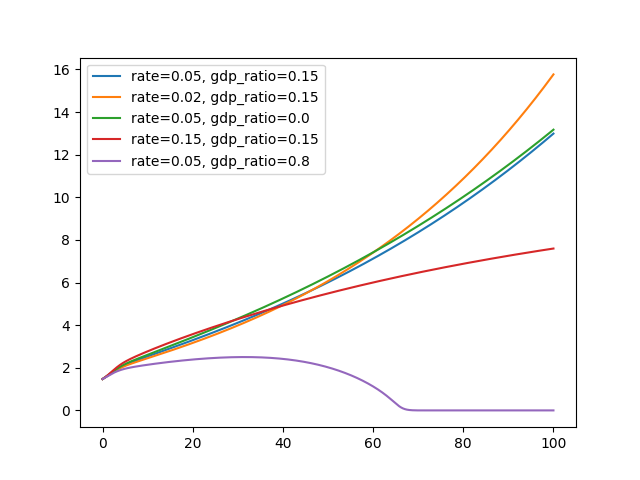
\includegraphics[width=1\textwidth]{output_per_labor_100}
\caption{\(\alpha=.3\), \(\sigma=.5\), \(\lambda=0\), \(q=0\).  \label{fig5}}
\end{minipage}\hfill
\begin{minipage}[t]{.48\textwidth}
\centering
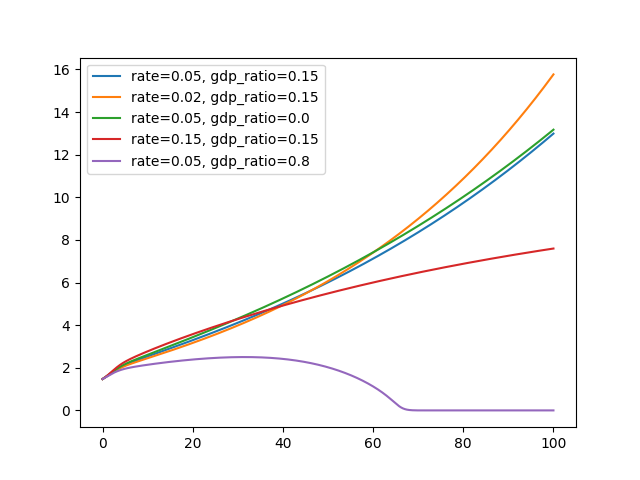
\includegraphics[width=1\textwidth]{output_per_labor_100}
\caption{\(z_0=1\), \(T=1\)  \label{fig6}}
\end{minipage}\hfill
\end{framed}
\end{figure}

\section{Numerical Inversion}




\section{Conclusion}



\newpage
\begin{thebibliography}{9}
\bibitem{baselii}
Basel Committee on Banking Supervision. International Convergence of Capital
Measurement and Capital Standards: A Revised Framework. Technical
report, Bank for International Settlements, 2006.
\bibitem{black1976}
F. Black and J. C. Cox. Valuing corporate securities: Some effects of bond
indenture provisions. \textit{Journal of Finance}, 31, 1976.
\bibitem{creditriskplus}
Credit Suisse. Creditrisk+: A credit risk management framework. Technical
report, Credit Suisse First Boston, 2001.
\bibitem{CIR1985}
J. C. Cox, J.E. Ingersoll, and S.A. Ross.  A Theory of the Term Structure of Interest Rates.  \textit{Econometrica}, 53, 1985.

\bibitem{duffie2005}
D. Duffie. Credit risk modeling with affine processes. \textit{Journal of Banking and Finance}, 29, 2005.
\bibitem{duffieBook2001}
D. Duffie. \textit{Dynamic Asset Pricing Theory}. Princeton University Press,
Princeton, New Jersey, third edition, 2001.
\bibitem{duffie1996}
D. Duffie and R. Kan. A yield-factor model of interest rates. \textit{Mathematical
Finance}, 6, 1996.
\bibitem{dufresne2001}
D. Dufresne. \textit{The integrated square-root process}. Number 90 in Research
Paper. Centre for Actuarial Studies, Department of Economics, University
of Melbourne, 2001.
\bibitem{fang2008}
F. Fang and C.W. Oosterlee. A novel pricing method for european options
based on fourier-cosine series expansions. \textit{SIAM Journal on Scientific Computing},
31, 2008.

\bibitem{Fok2014}
Pak-Wing Fok, Xiuling Yan, and Guangming Yao. Analysis of credit portfolio
risk using hierarchical multi-factor models. \textit{Journal of Credit Risk}, 10, 2014.
\bibitem{heston1993}
Steven Heston.  A Closed-Form Solution for Options with Stochastic Volatility with Applications to Bond and Current Options.  \textit{The Review of Financial Studies}, 6, 1993.
\bibitem{Hewitt1965}
E. Hewitt and K.R. Stromberg.  \textit{Real and Abstract Analysis}.  Springer-Verlag, New York, 1965.
\bibitem{jarrow1995}
R. A. Jarrow and S. Turnbull. Pricing derivatives on financial securities
subject to credit risk. \textit{Journal of Finance}, 50, 1995.
\bibitem{merton1974}
R. C. Merton. On the pricing of corporate debt: The risk structure of interest
rates. \textit{Journal of Finance}, 29, 1974.
\bibitem{creditmetrics}
J.P. Morgan. Creditmetrics. Technical report, J.P. Morgan, 1997.
\bibitem{oksendal2007}
Bernt Oksendal.  \textit{Stochastic Differential Equations}.  Springer-Verlag Berlin Heidelberg, sixth edition, 2007.
\bibitem{tasche2007}
D. Tasche and C. Acerbi. Euler allocation: Theory and practice. \textit{Zentrum
Marhematic (SCA)}, 2007.
\bibitem{vasicek1977}
O. Vasicek. An equilibrium characterization of the term structure. \textit{Journal of Financial Economics}, 5, 1997.
\bibitem{vasicek1987}
O. Vasicek. Probability of loss on loan portfolio. \textit{KMV Corporation}, 1987.
\bibitem{vasicek1997}
O. Vasicek. The loan loss distribution. \textit{KMV Corporation}, 1997.


\end{thebibliography}


\end{document}